% Created 2017-03-20 Mon 11:06
% Intended LaTeX compiler: pdflatex
\documentclass[11pt]{article}
\usepackage[utf8]{inputenc}
\usepackage[T1]{fontenc}
\usepackage{graphicx}
\usepackage{grffile}
\usepackage{longtable}
\usepackage{wrapfig}
\usepackage{rotating}
\usepackage[normalem]{ulem}
\usepackage{amsmath}
\usepackage{textcomp}
\usepackage{amssymb}
\usepackage{capt-of}
\usepackage{hyperref}
\usepackage[margin=1.2in]{geometry}
\usepackage{setspace}
\onehalfspacing
\usepackage{parskip}
\usepackage{booktabs}
\setcounter{secnumdepth}{2}
\author{Zheng Tian}
\date{}
\title{Replication of Examples in Chapter 4}
\hypersetup{
 pdfauthor={Zheng Tian},
 pdftitle={Replication of Examples in Chapter 4},
 pdfkeywords={},
 pdfsubject={},
 pdfcreator={Emacs 25.1.1 (Org mode 9.0.3)},
 pdflang={English}}
\begin{document}

\maketitle
\setcounter{tocdepth}{1}
\tableofcontents


\section{Introduction}
\label{sec:orge5a86ff}
This document is to show how to estimate a simple regression model and
perform linear hypothesis testing. The application concerns the test
scores of the California school districts. We will use R to estimate
the simple regression model with the data set in Chapter 4.

Before running all R codes, we may first load the package \texttt{AER} for
loading several particular packages of regression.
\begin{verbatim}
library(AER)
\end{verbatim}

\section{Reading the data and basic summary statistics}
\label{sec:org0412e52}
Let's first read the data into R and show some basic statistics.
\subsection{Read the data file}
\label{sec:orgb27d5b6}
The textbook comes with two files for the California test score data
set, \texttt{caschool.xlsx} and \texttt{caschool.dta}, the former of which is an
Excel file and the latter is a Stata file. We need to read either one
of these two files into R so that we can use the data set.

R has several built-in functions that can read an ASCII data file,
which can have such an extension as \texttt{.txt}, \texttt{.csv}, \texttt{dat}, to name a
few. However, these built-in functions cannot handle an Excel file or
a Stata file. So, in order to read \texttt{caschool.xlsx} or \texttt{caschool.dta}
in to R, we need additional packages.

To read a State file with an extension of \texttt{.dta}, we use the function,
\texttt{read.dta}, in the library of \texttt{foreign}.

\begin{verbatim}
library(foreign)
classdata <- read.dta("./data/caschool.dta")
\end{verbatim}

\texttt{classdata} is a dataframe object in R. If you want to check whether
your reading is correct, you can type  \texttt{head(classdata)}, which, by
default, displays the first six observations of all variables in the
data frame object.

\begin{verbatim}
head(classdata[c("observat", "district", "testscr", "str")])
\end{verbatim}

\begin{verbatim}
  observat                        district testscr      str
1        1              Sunol Glen Unified  690.80 17.88991
2        2            Manzanita Elementary  661.20 21.52466
3        3     Thermalito Union Elementary  643.60 18.69723
4        4 Golden Feather Union Elementary  647.70 17.35714
5        5        Palermo Union Elementary  640.85 18.67133
6        6         Burrel Union Elementary  605.55 21.40625
\end{verbatim}


\subsection{Summary}
\label{sec:orgacf70f1}

Upon reading the data, we often use \texttt{summary()} to see some basic
statistics. Here we are not going to show summary statistics of all
variables in the data set for the purpose of saving space, but only to
select several variables of interest in Chapters 4, including
test scores, \texttt{testscr}, student-teacher ratio, \texttt{str}.

\begin{verbatim}
df <- classdata[c("testscr", "str")]
summary(df)
\end{verbatim}

\begin{verbatim}
   testscr           str
Min.   :605.5   Min.   :14.00
1st Qu.:640.0   1st Qu.:18.58
Median :654.5   Median :19.72
Mean   :654.2   Mean   :19.64
3rd Qu.:666.7   3rd Qu.:20.87
Max.   :706.8   Max.   :25.80
\end{verbatim}

Formally, we can create a table showing important summary statistics,
like the following table (Table 4.1 in the book).\footnote{To create such a table, I use the function \texttt{xtable} in the
package of \texttt{xtable}, which generates a LaTex table. Also, I modified
the format of the LaTex table using the LaTex package
\texttt{booktabs}. LaTex is a typsetting system, like Microsfot Word, that is
capable of creating professional looking-like documents. Though LaTex
is not required for this course, learning it would be a great benefit
for your future career development, especially in academia}

\begin{verbatim}
# Replicate the summary statistics in Table 4.1
summary4.1 <- function(df){
    ave <- sapply(df, mean)
    std <- sapply(df, sd)
    perctile <- sapply(df, function(x)
	quantile(x, probs=c(0.1, 0.25, 0.4, 0.5, 0.6, 0.75, 0.9)))
    return(rbind(ave, std, perctile))
}
library(xtable)
sumtab <- xtable(t(summary4.1(df)))
\end{verbatim}

In the above code, I defined a function called \texttt{summary4.1}. In R, we
use \texttt{function()} to define a custom function. In this case, the
function \texttt{summary4.1} takes one argument \texttt{df}. The code within the
function is enclosed with the curly braces, \texttt{\{ \}}, and what the
function yields is controlled by \texttt{return()} in the last line.

Within the function \texttt{summary4.1}, I use a special function in R,
\texttt{sapply()}. It takes each component in a list object, which is \texttt{df} in
this case, and impose a function on this component, and return a
simplified object. Check the help information for \texttt{apply()},
\texttt{lapply()}, \texttt{sapply()}, \texttt{mapply()}, and \texttt{tapply()}.

Finally, the function \texttt{xtable()} writes the matrix that contains the
summary statistics into a table in either a \LaTeX{} or an HTML file.

\begin{verbatim}
print(sumtab, type = "latex")
\end{verbatim}

% latex table generated in R 3.3.2 by xtable 1.8-2 package
% Mon Mar 20 10:47:49 2017
\begin{table}[ht]
\centering
\begin{tabular}{rrrrrrrrrr}
  \hline
 & ave & std & 10\% & 25\% & 40\% & 50\% & 60\% & 75\% & 90\% \\
  \hline
testscr & 654.16 & 19.05 & 630.40 & 640.05 & 649.07 & 654.45 & 659.40 & 666.66 & 678.86 \\
  str & 19.64 & 1.89 & 17.35 & 18.58 & 19.27 & 19.72 & 20.08 & 20.87 & 21.87 \\
   \hline
\end{tabular}
\end{table}


\subsection{Create a scatterplot using \texttt{plot()}}
\label{sec:orgc1eac20}
It is always a good practice to make a scatterplot between an
independent variable and a dependent variable before setting up a
regression model. Let's draw a scatterplot of student-teacher ratios
and test scores. \texttt{plot} is the most basic function in R to draw
figures. Here I use it to draw the scatterplot as follows.

\begin{verbatim}
plot(df$str, df$testscr, col = "blue", pch =16, cex = 0.7, bty = "l",
     main = "Scatterplot of Test Score vs. Student-Teacher Ratio",
     xlab = "Student-teacher ratio", ylab = "Test scores")
\end{verbatim}

\begin{figure}[htbp]
\centering
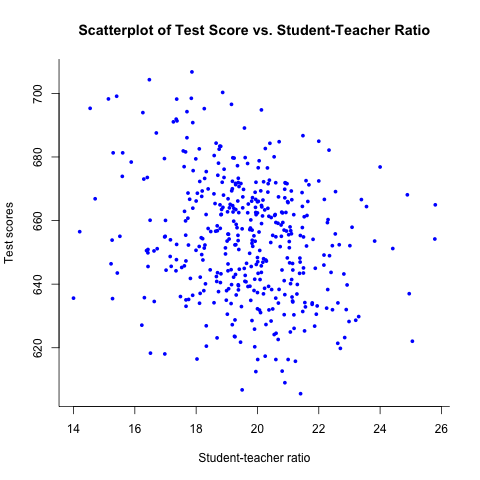
\includegraphics[width=0.85\textwidth]{fig42.png}
\caption{The scatterplot between student-teacher ratios and test scores}
\end{figure}

We can compute the correlation coefficient
between the two variables, using the function \texttt{cor}. Typing the
command \texttt{cor(df\$str), df\$testscr\}} yield the value of
\texttt{-0.23}.

\section{The OLS estimation}
\label{sec:org1657707}
\subsection{Set up the linear regression model}
\label{sec:org6918b90}

We establish the following linear regression model for the relationship between
test scores and class sizes
\begin{equation}
\label{eq:testscr-str-1}
TestScore_i = \beta_0 + \beta_1 STR_i + u_i
\end{equation}

\subsection{Estimate in R}
\label{sec:orga7b75df}
The OLS estimation can be implemented in R with the function \texttt{lm}. The
most important argument in this function is the model to be estimated,
which is called a \textbf{formula} object in R. A formula is defined using
the format \texttt{y \textasciitilde{} x1 + x2}, in which the symbol of \texttt{\textasciitilde{}} links the
left-hand side variable, \texttt{y}, and the right-hand side variables, \texttt{x1,
x2}. We can add more independent variables in the right-hand side with
each being appended to the formula by the symbol of \texttt{+}. The constant
term is by default included in the model. After estimation, we use
\texttt{summary} to see the results.

\begin{verbatim}
mod1 <- lm(testscr ~ str, data = df)
summary(mod1)
\end{verbatim}

\begin{verbatim}
Call:
lm(formula = testscr ~ str, data = df)

Residuals:
    Min      1Q  Median      3Q     Max
-47.727 -14.251   0.483  12.822  48.540

Coefficients:
            Estimate Std. Error t value Pr(>|t|)
(Intercept) 698.9330     9.4675  73.825  < 2e-16 ***
str          -2.2798     0.4798  -4.751 2.78e-06 ***
---
Signif. codes:  0 ‘***’ 0.001 ‘**’ 0.01 ‘*’ 0.05 ‘.’ 0.1 ‘ ’ 1

Residual standard error: 18.58 on 418 degrees of freedom
Multiple R-squared:  0.05124,	Adjusted R-squared:  0.04897
F-statistic: 22.58 on 1 and 418 DF,  p-value: 2.783e-06
\end{verbatim}

For now, we just pay attention to the estimates of the two
coefficients, which is \texttt{698.93} for the
intercept, \(\beta_{\text{0}}\), and \texttt{-2.28} for the slope.

\[\widehat{TestScore} = 698.93 - 2.28 \times STR\]

\subsection{Plot the sample regression line}
\label{sec:org5984265}
The sample regression line can be added to the scatterplot by using
the function \texttt{abline}. And an annotation can be added by using the
function \texttt{text}

\begin{verbatim}
plot(df$str, df$testscr, col = "blue", pch =16, cex = 0.7, bty = "l",
     xlab = "Student-teacher ratio", ylab = "Test scores")
abline(coef(mod1)[1], coef(mod1)[2], col="red")
text(23.5, 655, "TestScore = 698.9 - 2.28 STR", cex.lab = 0.9, font.lab = 3)
\end{verbatim}

\begin{figure}[htbp]
\centering
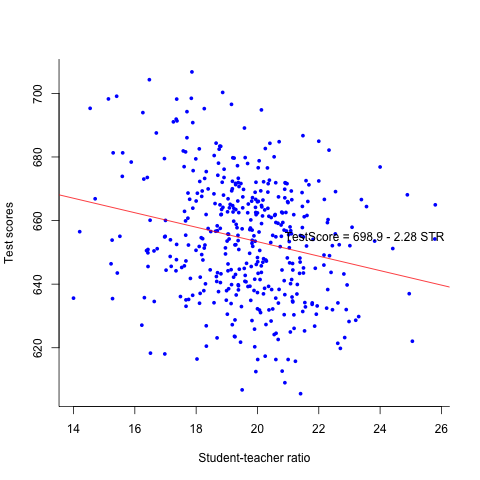
\includegraphics[width=0.75\textwidth]{fig43.png}
\caption{The estimated regression line for the California data}
\end{figure}
\end{document}